%-----------------------------------------------%
% Início do plano de aula
%-----------------------------------------------%
\thispagestyle{empty}
\begin{center}
	\begin{minipage}[!]{\linewidth}
        \begin{minipage}[!]{.19\linewidth}
            
\includegraphics[width=\linewidth]{img/logo.png}           
        \end{minipage}
        \begin{minipage}[!]{.8\linewidth}
            \center
            \ABNTEXchapterfont\normalsize\MakeUppercase{\imprimirinstituicao}
            \par
            \vspace*{10pt}                     
            \ABNTEXchapterfont\normalsize\MakeUppercase{\centro}
            \par
            \vspace*{10pt}           
            \ABNTEXchapterfont\normalsize\MakeUppercase{\disciplina}
        \end{minipage}        
    \end{minipage}
    \\ \vspace{0.5cm}
    \rule{\textwidth}{.5pt}   
\end{center}
    \textual
    \begin{center}
      \section{Fenômenos Ondulatórios I}
      \par
    \end{center}
    
    \noindent \textbf{Estagiário(a): }\imprimirautor 
    
    \noindent \textbf{U.E.: }EEB Giovani Pasqualini Faraco
    
    \noindent \textbf{Série: }2º Ano\hfill{}\textbf{Turma: }2º--5
    
    \noindent \textbf{Aula:} 007\hfill{}\textbf{Data:} 11/11/2022\hfill{}\textbf{Duração:} $45\min$
    \rule{\textwidth}{.5pt}
    \bigskip{}  
    

    \noindent
    \begin{center}
      \textbf{Interferência, difração e ressonância}
    \par\end{center}
    \vspace{20pt}
    \noindent \textbf{Resumo da aula:} Nesta aula apresentaremos de início, os argumentos fundamentais para a aceitação do modelo ondulatório da luz. Veremos que esta atribuição recebe ainda mais força após estabelecida a teoria eletromagnética de Maxwell, na sequência mostraremos, por meio de vídeos, os fenômenos ondulatórios relacionados a ressonância de ondas mecânicas e posteriormente apresentaremos o experimento de Hertz.
    \smallskip
    \par\noindent \textbf{Habilidades BNCC:} EM13CNT201.
    \medskip
    \subsection*{Objetivo de Aprendizagem}
    \begin{itemize}
        \item Conhecer exemplos do fenômeno de ressonância de ondas mecânicas e eletromagnéticas;
        \item Compreender o principal argumento a favor da concepção da luz como uma onda eletromagnética;
        \item Perceber as diversas formas de construção do conhecimento científico.
    \end{itemize}    
    \bigskip{}    
    \noindent \textbf{Núcleo Conceitual:} \emph{Fenômenos ondulatórios; luz como uma onda eletromagnética; experimento de Hertz.}
    \newpage
    

    \section*{Procedimento Didático} 
    \noindent\emph{1º Momento:} A Problemática da Aceitação Inicial de um Novo Modelo Científico
    \par\noindent\rule{.3\textwidth}{.5pt}  
    \par\noindent\textbf{Tempo previsto:} 10 minutos
    \smallskip
    \par\noindent\textbf{Dinâmica:} Iniciar comentando os resultados obtidos na aula anterior pela Lei de Snell. Perguntar se com o que foi visto até agora é possível fazer alguma afirmação para a natureza da luz, no que concerne ela pertencer ou não a algum dos modelos vistos.
    
    
    Citar que não havia, no entanto nenhuma comprovação experimental que denunciasse de fato a real natureza da luz. E que por mero prestígio devotado à figura de Newton, a teoria corpuscular segue sendo aceita como a descrição "correta" para os fenômenos luminosos, isto deixa o modelo ondulatório "silenciado" por cerca de 200 anos, até que Young quebra este silêncio com o experimento de fenda dupla.

    Iniciar a sequência de slides




% Segundo os autores é nessa etapa que se apresentam questões
% e/ou situações para discussão com os alunos, visando relacionar o estudo de um conteúdo com
% situações reais que eles conhecem e presenciam, mas que não conseguem interpretar completa ou
% corretamente porque provavelmente não dispõem de conhecimentos científicos suficientes. Ou seja,
% é na problematização que se deseja aguçar explicações contraditórias e localizar as possíveis
% limitações do conhecimento que vem sendo expressado, quando este é cotejado com o conhecimento
% científico que já foi selecionado para ser abordado (Delizoicov, Angotti e Pernambuco, 2002, p. 201).
% Portanto, esse primeiro momento é caracterizado pela compreensão e apreensão da posição dos alunos
% frente ao tema. É desejável ainda, que a postura do professor se volte mais para questionar e lançar
% dúvidas sobre o assunto que para responder e fornecer explicações.

    \bigskip{}
    \noindent\emph{2º Momento:} Organização do Conhecimento
    \par\noindent\rule{.3\textwidth}{.5pt}  
    \par\noindent\textbf{Tempo previsto:} 15 minutos
    \smallskip
    \par\noindent\textbf{Dinâmica:} Usando a sequência de slides, explicar o experimento de fenda dupla conduzido por Young e introduzir o conceito de interferência construtiva e destrutiva. Explicar também a difração por um orifício o que permitiu a Young obter, naquela época, dois feixes de luz coerentes entre si.  
    

    \noindent\textbf{Embasamento para os Slides}
    O experimento de fenda dupla, traz uma comprovação da luz como uma onda, haja visto que não há forma alguma de adequar este fenômeno dentro do modelo corpuscular, no entanto, abre-se uma nova questão -- \emph{se a luz é uma onda, que tipo de onda ela é?} Todas as ondas conhecidas até então, estavam enquadradas no escopo das ondas mecânicas governadas pelas leis de Newton, convém mencionar que para a época, uma das características primordiais das ondas de quaisquer natureza, é a necessidade de um meio físico para se propagar, como só se conheciam ondas de natureza mecânica, estes meios geralmente eram o ar, água, terra, cordas, molas e etc. 

    Paralelamente, especulações sobre a velocidade da luz tem sido feita desde os gregos, mas somente por volta do ano de 1670, Ole RØmer obteve um valor para esta velocidade ($c=212\kmps$) baseado em observações dos eclipses das luas de Júpiter. Após RØmer, Fizeau, desta vez experimentalmente, também obtém um valor para a velocidade da luz o que em 1849 Focault, com excelente precisão para a época, atualiza os resultados de Fizeau demonstrando que $c=298\kmps$.

    Ao mesmo tempo em que se desenvolvia técnicas mais precisas para medir a velocidade da Luz, uma teoria para o eletromagnetismo também ia ganhando espaço com James Clerk Maxwell. No desenvolvimento do eletromagnetismo, Maxwell previu a existência de um tipo de onda tal que a velocidade de propagação desta onda, coincide em alto grau com o valor da velocidade da luz obtida pelos experimentos mais precisos da época, no entanto, o eletromagnetismo recém teorizado carecia de comprovação. Fato dado por Heinrich Hertz em 1883.

    A importância dos experimentos de Hertz para o Eletromagnetismo de Maxwell, não apenas comprova experimentalmente a existência das ondas eletromagnéticas como também torna possível a inferência da luz visível como uma classe deste tipo de onda, o próprio Maxwell afirma em 1862 que:

    \begin{citacao}
        ``A velocidade das ondas transversais em nosso meio hipotético, calculada a partir dos experimentos electromagnéticos dos Srs. Kolhrausch e Weber, concorda tão exatamente com a velocidade da luz, calculada pelos experimentos óticos do Sr. Fizeau, que é difícil evitar a inferência de que a luz consiste nas ondulações transversais do mesmo meio que é a causa dos fenômenos elétricos e magnéticos.'' \cite{NUSSENZVEIG31997}
    \end{citacao}

    % https://www.youtube.com/watch?v=jUHgIYNEzJQ

    % https://cref.if.ufrgs.br/?contact-pergunta=leis-de-maxwell-e-ondas-eletromagneticas

    % https://cref.if.ufrgs.br/?contact-pergunta=como-a-luz-viaja-a-300-000-kms

    % https://cref.if.ufrgs.br/?contact-pergunta=leis-de-maxwell-e-ondas-eletromagneticas

    % http://www.virtual.ufc.br/solar/aula_link/SOLAR_2/Curso_de_Graduacao_a_Distancia/LFIS/A_a_H/Fisica_IV/aula_04/01.html

% Delizoicov e Angotti (1990, p. 29) explicam que nesse
% segundo momento os conhecimentos de Física necessários para a compreensão do tema e da
% problematização inicial devem ser sistematicamente estudados sob orientação do professor.
% Definições, conceitos, relações, leis, apresentadas no texto introdutório, serão agora aprofundados.
% De acordo com Albuquerque, Santos e Ferreira (2015, p. 467) esse é o momento em que os
% conhecimentos científicos passam a ser incorporados nas discussões. Os alunos começam a
% desenvolver uma compreensão a respeito da problematização ou situação inicial. Entretanto, para que
% isso ocorra, materiais devem ser consultados e atividades devem ser sugeridas para complementar as
% discussões, no sentido de incentivar e melhorar a sistematização dos conhecimentos.
% Nessa perspectiva, Delizoicov e Angotti (1990) vêm ressaltar a importância de diversificadas
% atividades, com as quais se poderá trabalhar para organizar a aprendizagem. Sugerem exposições,
% pelo professor, de definições e propriedades, além de formulações de questões (exercícios de fixação
% como dos livros didáticos), textos e experiências. Neste sentido, atualmente poderíamos acrescentar
% as mídias tecnológicas, como televisão, vídeos, filmes, programas tecnológicos, aplicativos de
% celulares, simulações, entre outros, de modo a auxiliar no processo da sistematização do
% conhecimento.

    \bigskip
    \noindent\emph{3º Momento:} Aplicação do Conhecimento
    \par\noindent\rule{.3\textwidth}{.5pt}  
    \par\noindent\textbf{Tempo previsto:} 20 minutos
    \smallskip
    \par\noindent\textbf{Dinâmica:} Apresentar os fenômeno de ressonância, por meio dos vídeos. Os dois primeiros vídeos abordam exemplos bem conhecidos sobre este fenômeno, a ressonância de ondas sonoras numa taça de cristal (Figura --\autoref{fig:ressonancia-cristal}) e a queda da ponte de Tacoma (Figura --\autoref{fig:ressonancia-tacoma}).

    \vspace{10pt}
    \begin{figure}[!ht]        
        \centering              
        \subfloat[\label{fig:ressonancia-cristal}]{
            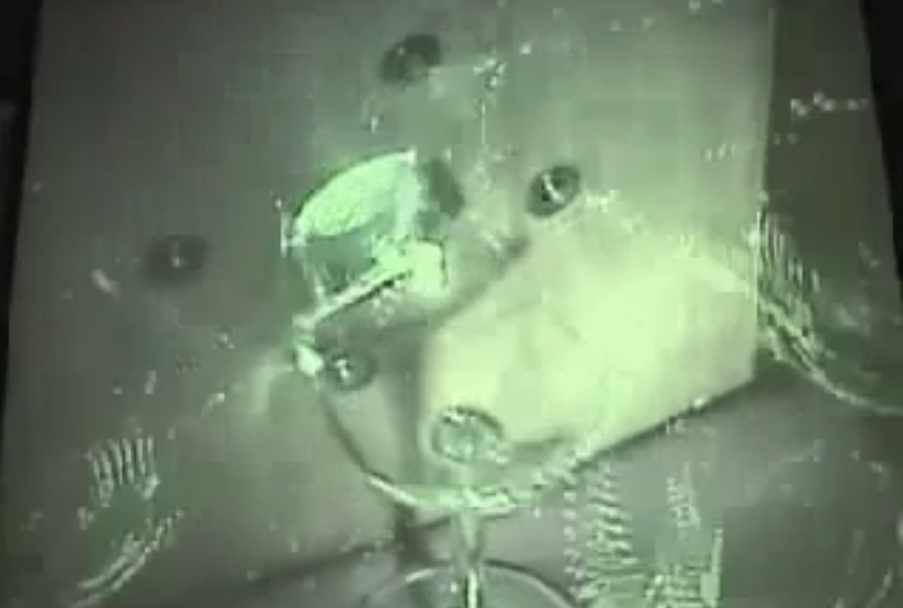
\includegraphics[width=.4\textwidth]{img/ressonancia-cristal.png}
        }\hspace{20pt}
        \subfloat[\label{fig:ressonancia-tacoma}]{
            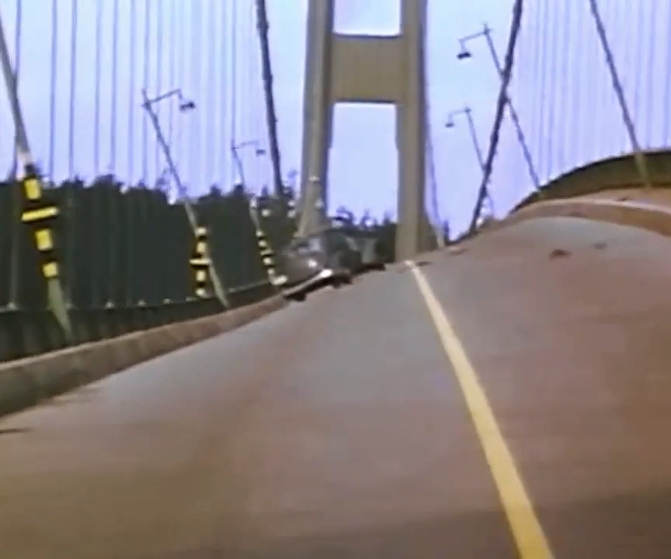
\includegraphics[width=.4\textwidth]{img/ressonancia-tacoma.png}
        }        
        \caption{Fenômenos de Ressonância: (a) Ressonância sonora numa taça de cristal ocorrendo segundos após a sua ruptura. (b) O famoso caso da ponte de Tacoma Narrows (1940)}
        \label{fig:ressonancia-1}
    \end{figure}        
    \vspace*{10pt}
    \newpage
    Após apresentar o fenômeno, mostrar o vídeo da ressonância em diapasões (Figura -- \autoref{fig:ressonancia-diapasoes}) o experimento deste vídeo é análogo ao experimento de Hertz (Figura -- \autoref{fig:ressonancia-hertz}) para as ondas eletromagnéticas.    
    \vspace{10pt}
    \begin{figure}[!ht]        
        \centering              
        \subfloat[\label{fig:ressonancia-diapasoes}]{
            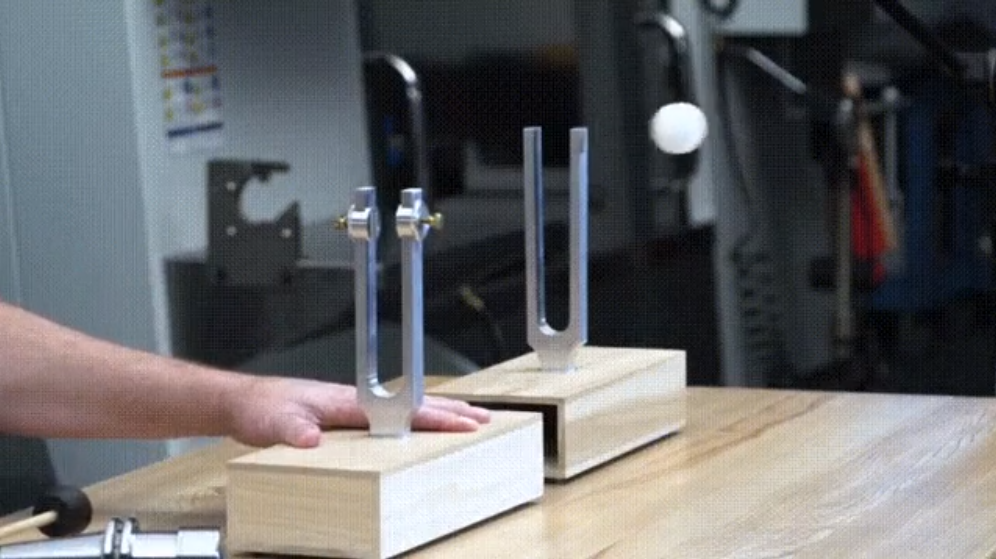
\includegraphics[width=.4\textwidth]{img/ressonancia-diapasao.png}
        }\hspace{20pt}
        \subfloat[\label{fig:ressonancia-hertz}]{
            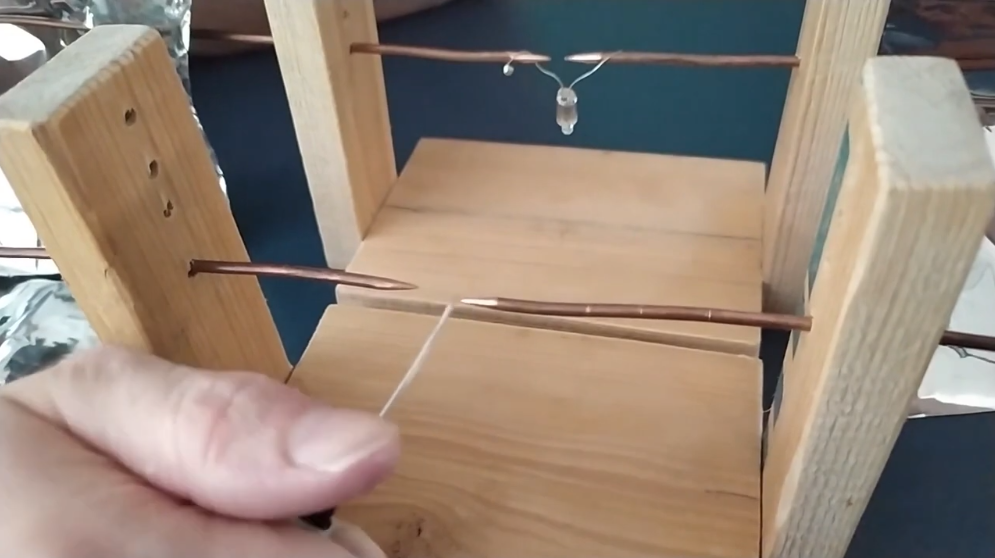
\includegraphics[width=.4\textwidth]{img/ressonancia-hertz.png}
        }        
        \caption{Fenômenos de Ressonância: (a) Ressonância sonora em diapasões. (b) Reprodução do experimento de Hertz}
        \label{fig:ressonancia-2}
    \end{figure}        
    \vspace*{10pt}

    Apresentar o experimento de Hertz como análogo ao fenômeno de ressonância entre diapasões.

    Questionar se conseguem encontrar alguma aplicação no cotidiano que se beneficie dos fenômenos de ressonância \emph{(transmissão de informações via ondas de radiofrequências; wi-fi; bluetooth; ressonância magnética e etc)}.

    Recuperar a aula enfatizando o que foi visto no vídeo do experimento de Hertz e realçar o caráter comprobatório dada ao experimento para adequar a luz como onda eletromagnética pela inferência da similaridade entre as velocidades destas ondas.
    

% Essa última etapa aborda sistematicamente o
% conhecimento que vem sendo incorporado pelo aluno para analisar e interpretar tanto a situações
% iniciais que determinaram o seu estudo, como outras situações que não estejam diretamente ligadas
% ao motivo inicial, mas que são explicadas pelo mesmo conhecimento. (Delizoicov e Angotti, 1990,
% p. 31).
% Este é o momento importante para que os alunos encontrem relações entre os temas
% abordados, não apenas através dos conceitos, mas também de fenômenos que possam ter alguma
% conexão com as informações apresentadas. No entanto, o professor mantém a postura
% problematizadora, podendo trazer questionamentos que não foram levantados pelos alunos, como
% informações e problemas que surgiram do decorrer dos momentos. Além disso, este é um bom
% momento para o professor formalizar alguns conceitos que não foram aprofundados pelos alunos.
% (Albuquerque, Santos e Ferreira, 2015).

%-----------------------------------------------%
% FIM do plano de aula
%-----------------------------------------------%